\section[Mitochondrial phylogenetic reconstruction]{Mitochondrial phylogenetic reconstruction - the power house of the phylogenies}
\label{cascade-sec:mitochondria}

While phylogenetic reconstruction is a well established method for genetic variants from canonical chromosomes to study metastatic progression and timing of evolutionary divergence \cite{Deshwar2015,Brown2017,Hu2019}, there are multiple issues. In \autoref{variantcalling-sec:phylo} and \autoref{variantcalling-sec:clonal} we showed how important the proper variant calling method is to accurately recover phylogenies and clonal patterns. In addition, using somatic variants to reconstruct phylogenies is a flawed concept flawed to begin with. Most models studying genetic variation assume neutral evolution of the sites \cite{Kimura1968,Lynch1989}, but cancers almost exclusively exhibit positive selection \cite{Cannataro2018}. And while passenger mutations might not directly affect fitness of the cell, they only exist due to the link to the driver mutation and therefore has little to no additional information gain in addition to the driver. In addition, while in small populations genetic drift as a stochastic process overpowers selective processes (fitness coefficient $s$) and can therefore be assumed to be neutral, in larger populations $N_e$ (effective population size) where \autoref{mmf-eq:neutralSelection} does not hold true, mutations are under selective pressure \cite{EyreWalker2007}.
\begin{equation}
N_e \cdot s \ll 1 \label{mmf-eq:neutralSelection}
\end{equation}
\myequation[\ref{mmf-eq:neutralSelection}]{Selective pressure with effective population size}
%we need to squish this a bit otherwise it looks weird
\vspace{-3em}
All in all we can assume that with cancer growing, positive selection through treatment and tumour micro environmental niches, almost all assumptions of the coalescent theory are not applicable for tumour samples and therefore methods using somatic variants and their respective results need to be selected and evaluated carefully.

To tackle this issue, and assist with the interpretation of phylogenetic reconstruction results, we adjusted a method used in single cell sequencing to track clonal expansion with mitochondrial somatic mutations \cite{Ludwig2019} to be usable for standard bulk sequencing. Mitochondrial variants are an ideal source of clonality information, because the mutation rate is significantly higher than nuclear DNA, due to the missing proof reading and repair mechanisms, which allows very granular separation in a shorter time period. Additionally, while there are several diseases cause by defects in mitochondria such as Kearns-Sayre syndrom \cite{Harvey1992}, MERRF \cite{Adam1993} and MELAS \cite{Hirano1992}, they usually follow a mendelian inheritance pattern and are hereditary and not somatically acquired. In the cancer text, somatic mutations in mitochondrial DNA are assumed to be approximately neutral with a possible selection pressure towards healthy ageing and negatively selecting cancer \cite{Rodell2013,Yuan2020}.

\subsection{Method}
\label{cascade-sec:mitoMethod}

First a pileup of all mitochondrial positions is performed. Before the pileup we preselect reads which uniquely map to the mitochondrial genome and only retain high mapping quality reads. Then the nucleotide counts in each position is transformed into a MultiEssayExperiment \cite{Ramos2017} for final analysis in R. The preprocessing code and be found in \autoref{lst-cascadeAppendix:mitoPreProcessing}.

The final MultiEssayExperiment is then read into R and quality metrics applied to exclude samples with not enough coverage on the mitochondrial contig. usually WGS samples will show an extensive coverage of mitochondrial DNA, however WES will require a library preparation with probes in this area. Patient CA-I has a coverage of more than 100x for all but the germline sample which only has an overall coverage of 17x. Similar, patient CA-L shows lower depth for the germline sample (127x) but a generally high coverage for all tumour samples. All other Patients (CA-A/J/K) where samples are sequenced as WGS show a coverage of more than 200 even for low performing samples with a median depth of \num{67916}, \num{45603} and \num{49726} per sample.

\begin{figure}[!ht]
\centering
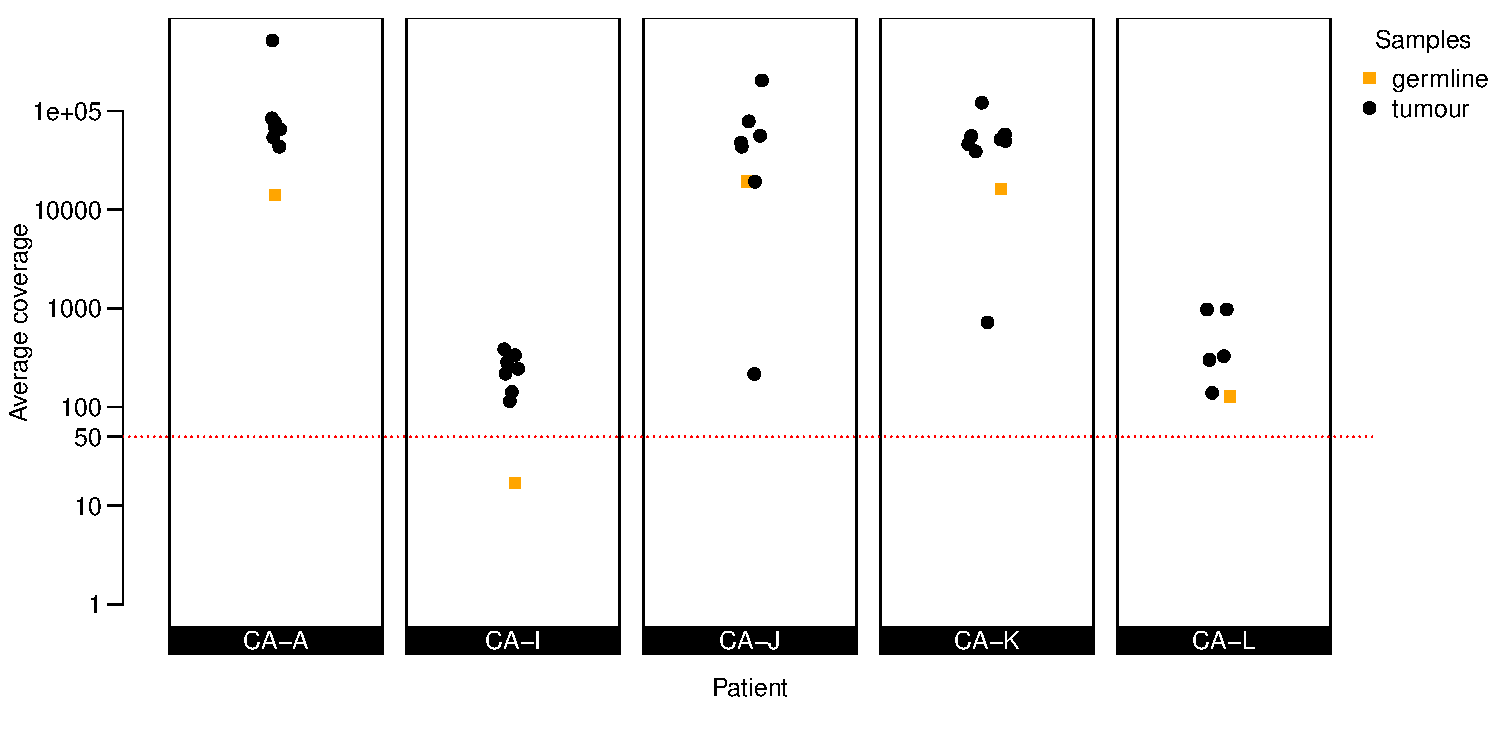
\includegraphics[width=.99\linewidth]{Figures/mtCoverage}
\vspace{-1em}
\caption[Average coverage of mitochondrial DNA of CASCADE patients]{Average coverage of mitochondrial DNA of CASCADE patients: Orange squares show germline sample for each patient; black points show tumour samples; horizontal red dotted line shows quality cut off suggested by \protect\textcite{Ludwig2019}} \label{fig:cas86schematic}
\end{figure}

This shows, that even without specifically enriching for mitochondrial DNA, most samples will contain enough tumour reads for this analysis.

To ensure optimal results, we excluded all samples with an average coverage of less than 50x. This means we remove the germline sample for patient CA-I, however as we expect the germline sample to be the ancestral state for all samples, so it can be reconstructed. Secondly, we were more interested in the relation of tumour samples with each other, which is still possible.

In contrast to the simple hamming distance used for the presence-absence vector representation of canonical somatic variants (\autoref{cascade-sec:phylo}) for mitochondrial variants we employed a allele frequency ($vaf$) based distance (\autoref{eq:mitoDist}) of two samples~$s_i$ and $s_j$. The difference in read support is normalised with the product of the total allelic depth~$cov$ and summed up at all sites of variation~$v$.

\begin{equation}
mitoDist(s_i,s_j) = \sum_{v \in Variants} \left| \frac{vaf_{s_i}(v) \cdot cov_{s_i}(v) - vaf_{s_j}(v) \cdot cov_{s_j}(v)}{cov_{s_i}(v) \cdot cov_{s_j}(v)} \right| \label{eq:mitoDist}
\end{equation}
\myequation[\ref{eq:mitoDist}]{Mitochondrial variants based distance function of two samples}

This distance was only calculated for variant sites where both samples had at least a coverage of 100x to have a representative sampling of the allelic prevalence in each sample as a human cell usually has more than 100 mitochondria \cite{Cole2016}.